\section*{Conclusione}

\subsection*{Transistor come interruttore veloce}

Il motivo per cui il LED si accende e si spegne è facilmente spiegabile in quanto: il terminale emettitore del transistor si trova ad un potenziale di $0\,\si{\volt}$. Quindi affinché possa passare corrente tra la base e l'emettitore occorre che tra queste vi sia una differenza di potenziale di almeno $0.6\,\si{\volt}$. Quindi dal momento che il segnale in ingresso permette sostanzialmente due valori di tensione di base ($V_b$), ovvero 0 e 5 $\si{\volt}$, allora quando $V_b=0\,\si{\volt}$ il ramo base-emettitore non conduce e nel circuito non passa corrente. Al contrario quando $V_b=5\,\si{\volt}$, allora il ramo base-emettitore entra in conduzione e nel circuito passa corrente e pertanto il LED si illumina.

\subsection*{Emitter follower}

Come è possibile osservare dalla Figura \ref{fig:emitter} notiamo che il circuito (c) ci permette di visualizzate in output solamente la parte di segnale dovuta alla semionda positiva, mentre la parte negativa del segnale viene completamente tagiata. Questo comportamento è analogo a quello visto nel punto precedente. Ovvero la condizione necessaria affinche passi corrente tra i terminali di base e emettitore del transistor è che devono essere polarizzati in diretta. Dal momento che la base del transistor si trova ad una tensione di $0\,\si{\volt}$ allora base ed emettitore si trovano in condizione di polarizzazione diretta soltanto quando il segnale in ingersso alla base ($V\ped{in}$) è di almeno 0.6 V. Al contrario (per $V\ped{in}\,\leq\,0.6\,\si{\volt}$) non abbiamo passaggio di corrente e pertanto $V\ped{out}$ risulta nullo.

\subsection*{Emitter follower polarizzato}

\begin{wrapfigure}{r}{0.5\textwidth}
    \vspace{-10mm}
    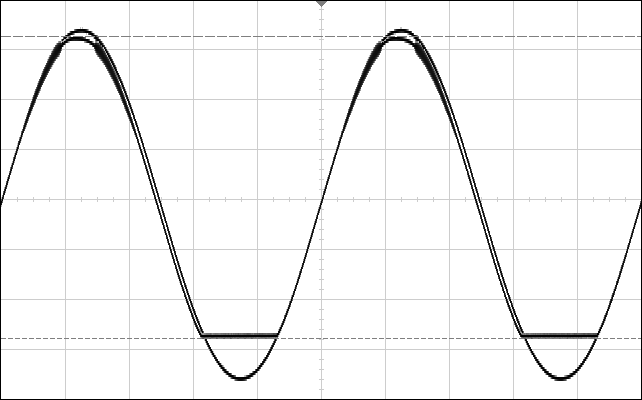
\includegraphics[width=0.5\textwidth]{clip.png}
    \vspace{-10mm}
\end{wrapfigure}

Come illustrato in Figura \ref{fig:emitter_b} in questa configurazione il nostro circuito permette di visualizzare in output ($V\ped{out}$) un segnale che è ``identico'' a quello in ingresso. Questo risultato differisce da quello ottenuto per un semplice emitter follower (analizzato nella sezione precedente), in quanto l'emettitore è collegato al terminale di tensione $-12\,\si{\volt}$. Questo comporta che, quando la base si trova ad una tensione $V\ped{in}\,\leq\,0\,\si{\volt}$, base ed emettitore risultano essere comunque polarizzati in diretta. Pertanto peremettono un passaggio di corrente anche quando il segnale è negativo.

Inoltre abbiamo osservato come si comporta $V\ped{out}$ al variare di $V\ped{in}$. Quello che abbiamo ottenuto è che, come visibile nella figura a fianco, quando l'ampiezza del segnale in ingresso è maggiore di circa 11.5 V, il transistor entra in interdizione per alcuni parti del segnale e quindi lo ``taglia''. Questo fenomeno è detto clamping.

\subsection*{Emitter follower come partitore di tensione}

La procedura con cui abbiamo dimensionato il circuito è descritta nella sezione di Analisi dati. Infine grazie a quanto osservato in laboratorio possiamo dire che, mantenendo costante l'ampiezza del segnale in ingresso $V\ped{in}$ e variandone la frequenza, man mano che quest'ultima aumenta cresce anche lo sfasamento tra il segnale in ingresso e in uscita, come ci si aspetta da un filtro passa-alto.
